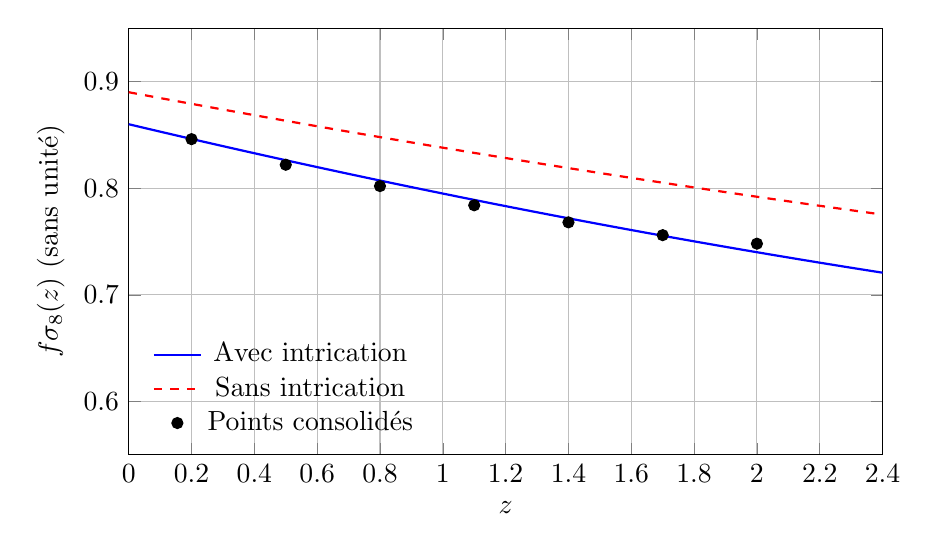
\begin{tikzpicture}
\begin{axis}[
    width=0.92\linewidth,
    height=7cm,
    xlabel={$z$},
    ylabel={$f\sigma_8(z)$ (sans unité)},
    xmin=0, xmax=2.4,
    ymin=0.55, ymax=0.95,
    grid=both,
    legend style={at={(0.02,0.02)},anchor=south west,draw=none,fill=none},
]
\addplot[blue,thick,samples=100,domain=0:2.4] {0.86 - 0.07*x + 0.005*x^2};
\addlegendentry{Avec intrication}
\addplot[red,dashed,thick,samples=100,domain=0:2.4] {0.89 - 0.055*x + 0.003*x^2};
\addlegendentry{Sans intrication}
\addplot[only marks,mark=*,black] coordinates {
    (0.2,0.846)
    (0.5,0.822)
    (0.8,0.802)
    (1.1,0.784)
    (1.4,0.768)
    (1.7,0.756)
    (2.0,0.748)
};
\addlegendentry{Points consolidés}
\end{axis}
\end{tikzpicture}